
\section{实验内容与设计}

\subsection{实验目的}
    \begin{enumerate}
        \item 了解滑动摩擦定律和静、动滑动摩擦系数的概念;
        \item 了解静、动滑动摩擦系数的测量原理和方法,测定并对比不同材质和工况下的静、
        动滑动摩擦系数;
        \item 实践基本的数据处理、分析以及书面报告表达。
    \end{enumerate}

\subsection{实验仪器}

    \begin{enumerate}
        \item JLT-1 理论力学多功能实验台;
        \item JLT-1 理论力学多功能实验台;
        \item 金属滑块、有机玻璃滑块;
        \item 不锈钢平板、铝合金平板。
    \end{enumerate}



\subsection{实验原理}
当两个相互接触的物体具有相对滑动趋势时,
在其接触界面处会产生阻碍相对运动的相互作用力,
这种力被定义为滑动摩擦力(Sliding friction force)。
滑动摩擦力的作用方向始终与接触面间的相对滑动趋势方向相反。
根据相对滑动趋势的发展程度,滑动摩擦力可处于静,动两种状态:
(1)当相对滑动趋势较小时,物体间保持相对静止状态,
此时产生的摩擦力称为静滑动摩擦力(Static sliding friction force)。
在此阶段,静滑动摩擦力的大小随外部作用力的增加而相应增大;
(2)当静滑动摩擦力达到其极限值而无法继续平衡外部作用力时,
物体间开始产生相对滑动,此时接触面间的摩擦力转变为动滑动摩擦力
(Kinetic sliding friction force)。
静滑动摩擦力所能达到的极限值被称为最大静滑动摩擦力
(Maximum static sliding friction force)。
由于除极限值以外的静滑动摩擦力不具有对物体接触界面状态的表征意义,
因此最大静滑动摩擦力常省略"最大"二字,简称为静滑动摩擦力。

库伦摩擦定律(Coulomb's law of friction)表明:当两物体相互滑动,
两物体间滑动摩擦力(记作 $F_d$ )正比于两物体接触处的正压力(记作 $N$ ),
即,$F_d=f_d \cdot N$ ,摩擦力方向与速度方向相反。
式中无量纲的系数 $f_d$ 称为动滑动摩擦系数,它与相对滑动速度无关,
仅取决于两物体接触面的材质与表面情况。
处于静-动临界状态的最大静滑动摩擦力(记作 $F_{\text {max }}$ )
同样仅取决于正压力和两物体接触面材质与表面情况,
因此可以相同形式描述:$F_{\max }=f_s \cdot N$ ,
式中无量纲的系数 $f_s$ 称为静滑动摩擦系数。    

依据摩擦理论,对于相同的两物体及其接触面状态,两滑动摩擦系数 $\left(f_d, ~ f_s\right)$ 应保持为常数。
由于摩擦的机理涉及接触面复杂的弹塑性变形乃至微观层面的分子作用,
人们很难通过现有理论准确计算出滑动摩擦系数,
一般需要借助实验方法进行近似测定。

本实验通过滑块和可调倾角的平板来测定物体的静,动滑动摩擦系数。
实验装置如图 1 所示。(最大)静滑动摩擦系数和动滑动摩擦系数的测量原理如下:

\subsection{(最大)静滑动摩擦系数测量}
预先设置较大的平板坡度,使滑块可以在平板上顺利下滑。通过升降手柄逐步降低平板倾斜角 $\varphi$ ,直至滑块保持静止,记录此时的平板倾斜角 $\varphi_s$ 。根据力的平衡有:

$$
\left\{\begin{array}{l}
F_{\max }=G \cdot \sin \varphi_s \\
N=G \cdot \cos \varphi_s
\end{array} \Rightarrow f_s=\frac{F_{\max }}{N}=\tan \varphi_s\right.
$$

\begin{figure}[h!]
    \centering
    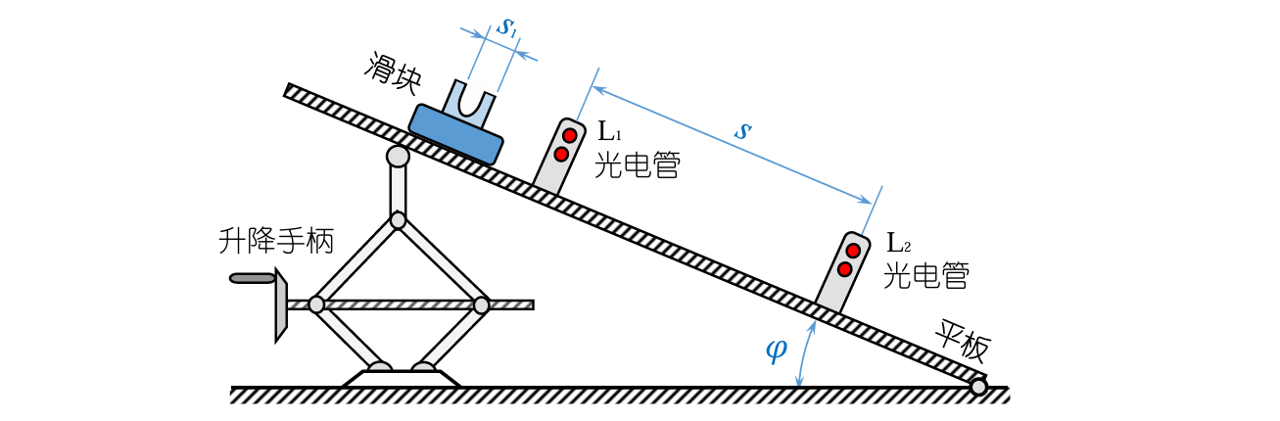
\includegraphics[width=\textwidth]{image/滑动摩擦系数测量装置示意图.png}
    \caption{滑动摩擦系数测量装置示意图}
\end{figure}

\subsection{动滑动摩擦系数的测量}

取倾斜角度 $\varphi>\varphi_s$ ,使得滑块可顺畅滑到平板底部。倾斜平板上有光电管 L1 和 L2,可检测固定于滑块上的相距 $s_1$ 的两挡板的抵达时间。测得两挡板相继扫过 L1 的时间间隔为 $t_1$ ,相继扫过 L 2 的时间间隔为 $t_2$ ,挡板最前锋扫过 L 1 和 L 2 的时间间隔为 $t_3$ ,那么,$s_1$ 中点通过 L1 和 L2 的时间间隔可近似表示为 $t_4=t_3+0.5\left(t_2-t_1\right)$ 。由此可计算得到滑块的平均加速度:

$$
a=\frac{V_2-V_1}{t_4}=\frac{\frac{s_1}{t_2}-\frac{s_1}{t_1}}{t_4}=\frac{s_1 \cdot\left(t_1-t_2\right)}{t_1 \cdot t_2 \cdot t_4}
$$


根据牛顿第二定律:

$$
\begin{gathered}
\left\{\begin{array} { l } 
{ \text { 平板切向:} \sum F _ { \tau } = m a } \\
{ \text { 平板法向:} \sum F _ { n } = 0 }
\end{array} \Rightarrow \left\{\begin{array}{l}
m g \sin \varphi-f_d \cdot N=m a \\
m g \cos \varphi-N=0
\end{array}\right.\right. \\
\Rightarrow \quad f_d=\frac{m g \sin \varphi-m a}{m g \cos \varphi}=\tan \varphi-\frac{a}{g \cos \varphi}
\end{gathered}
$$


将加速度代入,得到动滑动摩擦系数:

$$
f_d=\tan \varphi-\frac{s_1 \cdot\left(t_1-t_2\right)}{g \cdot t_1 \cdot t_2 \cdot t_4 \cdot \cos \varphi}
$$


   